\documentclass[a4paper,10pt]{article}
\usepackage[cm]{fullpage}
\usepackage{graphicx}
\usepackage[colorlinks=true,linkcolor=black,citecolor=black,filecolor=black,urlcolor=black]{hyperref}
\usepackage{acronym}

\acrodef{FIRA}{Federation of International Robot-soccer Association}
\acrodef{DLL}{Dynamic Link Library}
\acrodef{SIMD}{Single-Instruction Multiple-Data}

\begin{document}

\begin{titlepage}
  \setlength{\parindent}{0cm}

  
\includegraphics[width=200px]{Images/uob-logo-black-transparent}

  \Large
  Faculty of Engineering and Design

  \vspace{80pt}

  \LARGE
  Final Year MEng Project \\
  Project Plan and Literature Review

  \vspace{80pt}
  \textbf{Robot Football - High Level Control and Strategy Implementation}

  \vspace{10pt}
  \emph{Anthony Richards} \\
  \emph{\today}

  \vspace{80pt}
  Supervisor: \emph{Dr.~Pejman Iravani}

  \vspace{10pt}
  Assessor: \emph{TBD}
\end{titlepage}

\pagenumbering{roman}

\begin{abstract}
\acresetall
The aim of this project is to develop of a set of control algorithms for the \ac{FIRA} Middle Leage Simursot Game, a simulated five-a-side game played by small (not humanoid) autonomous robots.  A large amount of research has been performed in this and related fields, as a result of the \ac{FIRA} competitions, and this provides a good background of work from which to develop new or improved strategies. The main challenge of the project is to produce a set of systems that will work together to develop a suitable strategy, based on the current state of the system.  Work will also be done on using predictions of the future state of the system to improve this prediction. Support subsystems will then be required to implement the strategy, by determining how the robots must move to implement the strategy, and then algorithms to move the robot to the required position. A successful system will increase the chances of the team beating the default strategy provided by \ac{FIRA} compared to the strategy playing against itself.
\end{abstract}

\acresetall
\tableofcontents

\cleardoublepage
\acresetall

\pagenumbering{arabic}

\section{Project Background}
The \ac{FIRA} Middle League SimuroSot Game involves two teams of five simulated robots placed to play a form of five-a-side football against each other with minimal human intervention.  Based on the \ac{FIRA} MiroSot game, which uses five size restricted robots to play the game, the aim of SimuroSot is to allow development and competition of suitable strategies without requiring hardware to be produced to support it. \cite{simurosotSim}

The environment, set up to simulate the playing field as well as the robots and the playing ball, is shown in Figure \ref{fig:simulatorEnvironment}.  This environment then interfaces with a specified strategy file (either a Windows \ac{DLL} or a script file written in Lingo), and calls pre-specified functions to operate the strategies as the game continues.  The environment handles the simulation of the physics of the system, including the motion of every element as well as collisions and other interactions.

\begin{figure}
 \centering
 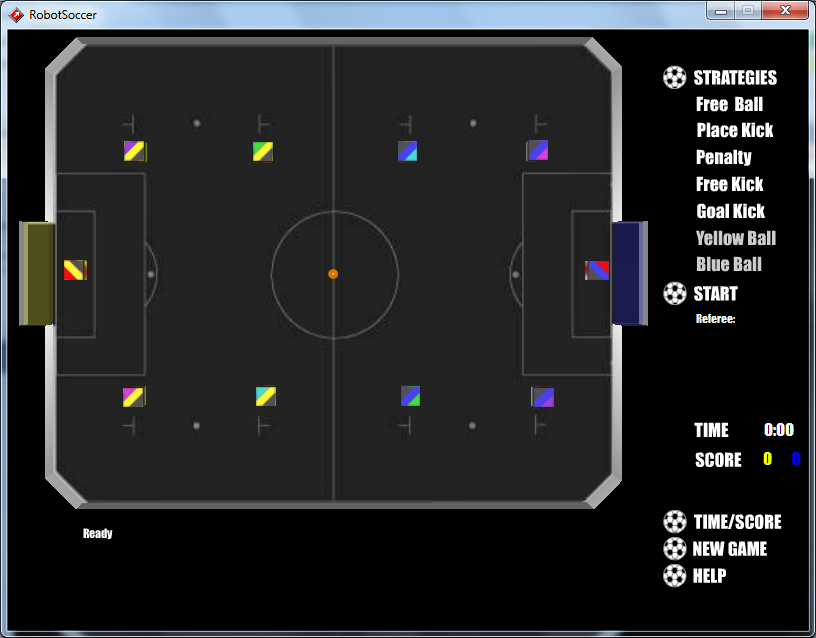
\includegraphics[width=0.6\textwidth]{Images/simulator-screenshot.png}
 \caption{SimuroSot Simulation Environment}
 \label{fig:simulatorEnvironment}
\end{figure}



The problem presented by the game has been investigated by many groups while competing in both the \ac{FIRA} leagues as well as the similar RoboCup games.  Many of the findings produced while investigating the physical games are equally applicable to the simulated version, as they handle high-level concepts encountered in both environments (such as route-finding or game strategy).

\subsection{Preliminary Literature Review}

The problem of having a team of separate entities successfully cooperate to achieve a goal is a common theme in multi-agent problems.  He, Ge and Tong consider the application of flocking algorithms to the problem, using the behaviours to first position the robots with respect to each other and the ball, and then control the group through the lead robot to score a goal \cite{taskBasedFlocking}.  Lee, Na and Kim consider a system that assigns specific roles that they pursue individually, depending on the current state of the game and their primary role \cite{taskRoleSelectionStrategy}, as do Hajduk and Sukop \cite{multiagentsDynamicBoxChange}. Artificial immune system techniques have been explored by Luh, Wu and Liu \cite{artificialImmuneSystemCooperation}, using the biomimetic technique to control the behaviour of each robot to produce the required cooperation.

All the techniques so far discussed take into account only the current state of the system, aiming to manoeuvre to take advantage of what is currently happening without any obvious attempt to predict the future state of the system.  There appears to be little literature on complete strategies that use predictions of the future state of the game to make decisions.

At a slightly more general level, Kok and Vlassis consider the methods of making decisions in a multi-agent system.  They use a graph to represent the problem space and then use the max-plus algorithm to select the best option available \cite{maxPlusAlgorithm}.  Dawei and Shiyuan use simulated annealing on similar graphs to derive a solution to the problem, using a method that can be interrupted if it runs out of time, while still producing a partial solution \cite{simulatedAnnealingDecisionMaking}.  Dorer has explored a more human-like method, using extended behaviour networks \cite{modellingHumanDecisionMaking}, which have seen success in some competitions.  These techniques all work by selected the option given the highest score out of all the possible options, but provide no detailed discussion on how these scores are calculated.

Kyrylov has explored weighing up the gains, costs and risks of making moves in the game, specifically looking at passing the ball \cite{balancingGainsRisksCostsPassing}.  The algorithm examines several possible outcomes of each action and uses a Pareto optimality approach to decide on the best option.  The techniques discussed could be useful for application to other decisions as well.

Proceeding to more abstract techniques, a lot of research has been done on the general tasks that need to be performed to achieve the goal.

Route finding and trajectory planning is a very common technique in this field.  The A* algorithm, a common system used to find paths, is described by Russel and Norvig \cite{aiModernApproach}.  This algorithm has been widely used to find paths in a discretised environment, and is also applicable to navigating graphs representing game moves to find an optimal set of decisions.  Alternatively, Bruce and Veloso have proposed a continuous route finding technique that avoids some of the non-optimal characteristics of the discretised algorithms like A* \cite{realTimeRandomizedPathPlanning}.

Multi-agent techniques have also been applied to route finding problems.  Particle swarm optimisation techniques are described by Sun and Xu \cite{psoForUAV}, Zhu, Qian, Li and Zhu \cite{psoRouting}, who also take into account time windows, and Chiou, Wang and Shieh \cite{fuzzyAntColony}, who present a more specialised version based on an ant colony.  The first paper is of particular interest as the algorithm also contains details on avoiding opponents (enemy combatents in the paper, but opposing players in this case).

Collision avoidance is another widely research technique.  Jacobs, Ferrein, Schiffer, et al propose a method utilising the A* to avoid static obstacles \cite{robustRealTimeRoutePlanning}.  Sarker, Shome and Nandy propose a combined route planning and obstacle avoidance algorithm which uses a variant of potential field force techniques to avoid obstacles \cite{intelligentAlgorithmPathPlanning}, while Lim, Kim, An and Kim propose one based on the limit-cycle navigation method, which has the robot move in a planned circle around obstacles \cite{limitCycleNavigation}.

If the algorithms are to work effectively, they need to be able to make a decision and act in a shorter time than the simulation time step.  If the strategy algorithms are complex, this means that they need to operate as fast as possible, taking full advantage of the features of the host processor.  A lot of research has been put into the optimal use of the \ac{SIMD} functions of a modern processor, as well as the multi-tasking capabilities of multiple-core devices.  Of particular interest is a set of application notes produced by Intel that provide good use of the \ac{SIMD} functions.  They have presented an efficient method of matrix inversion \cite{intelMatrixInverse}, as well as matrix multiplication \cite{intelMatrixMultiply} that can be useful for solving multiple simultaneous equations rapidly, a common task in motion planning and prediction,

\section{Aims and Objectives}
The aim of this project is to produce a set of algorithms that will allow a team of five robots to play a game of football against another team and win.  In order to achieve this, the following subsystems must be in place:

\begin{itemize}
\item A subsystem that will allow the robots to position themselves at an arbitrary position with a given final speed and direction of motion (within the limits of the robots).  This will allow the robots to interact with the ball to produce the motion required by the higher-level planning algorithms.

\item A subsystem that can predict the location of the ball or an opposing robot at a given time in the future.  The prediction will only need to work for the next two to three seconds, allowing better decisions to be made.

\item A subsystem that will monitor the behaviour of each robot and ensure that it's actions will not cause a foul (as described in the \ac{FIRA} rules of play \cite{simurosotSim}).  For example, it should intervene if an action will cause a collision with an opponent by altering a planned route appropriately.  This will ensure that the team is compliant with the rules and does not incur any corrective action from the referee.

\item A subsystem that will combine the previous two to produce a path for a robot to allow it to interact with the ball to change the balls speed and direction of motion.  This will allow the higher level planning sub-systems to state a desired ball motion path and have a robot cause that action to happen.

\item A subsystem that will take in the current state of the system and decide on an appropriate course of action. When the ball is under the control of the current player, it will have the robots attack the opposing goal and attempt to score a goal.  When the ball is under the control of the opposition it will attempt to defend its own goal and disrupt the opponents actions. When the ball is not under any defined control, it will attempt to take control of the ball.
\end{itemize}

The entire system must be sufficiently lightweight to allow all of it to be run once per simulator frame.  This will allow the system to respond quickly to the current state of the system and take advantage of any changes as soon as possible.

A successful system will be able to consistently perform better than the standard strategy provided with the SimuroSot simulator.  This can be measured by setting the two strategies against each other in the simulator and seeing which team wins.

If a successful system is produced, it may be possible to present it to the \ac{FIRA} competition happening this year in Bristol.  This will be dependent on the progress made, as the project will have restricted man-hours available for work compared to other teams in the SimuroSot league (as other teams usually consist of more than just one person).

\section{Methodology and Deliverables}
The main result of the project will be a SimuroSot simulator compatible \ac{DLL} containing the algorithms required to produce the desired strategy.  This \ac{DLL} can then be loaded by the simulator and the simulation run to observe the results.

As the documentation for the simulator is sparse, it will first be necessary to examine the behaviour of the system to confirm the underlying equations of motion and what (if any) simplifications have been made to the physics.  This information can then be used to produce the motion prediction algorithms, as well as the algorithms required to plan trajectories.

The initial attempt at high-level strategy will use a scoring system to determine which robots are in the best position to achieve the current goal (e.g. offence or ball interception).  These scores can then be used to produce a tree of possible outcomes, and a suitable algorithm can be used to select the best move.  This will attempt to take into account not just the current 'move', but also the next one, to best allow the system to plan ahead.

The system will be made as lightweight as possible by taking full advantage of the advanced features of modern processors that allow multiple actions to be achieved simultaneously (e.g. with multi-threading and \ac{SIMD} instructions as discussed in \cite{intelMatrixInverse}).  The profiling tools provided with Visual Studio will be used to confirm any perceived improvements.

The success of the system will be measured by comparing the behaviour of the system over a number of games (to allow for the effects of random chance) compared to the basic strategy playing against itself.  The best strategy would always beat the standard strategy, but one that creates a significant improvement on the chances of winning would still be a success.  If this is successful, the system will then be tested against any other algorithms that have been published (for example the sample algorithms produced by Nottingham University \cite{nottsWebsiteStrategy}).

\section{Resources}
As this project is targeted at the SimuroSot league, all the activities will be carried out in software only.  In order to produce the required software, the following software will be required:

\begin{itemize}
 \item Microsoft Visual Studio 2010
 \item SimuroSot Middle League Simulator
\end{itemize}

Visual Studio is available on the University computers in the Maxwell and Faraday labs in the Electrical Engineering Department, as well as on the GigaTerms server which is available via Remote Desktop.  It is also available free of charge to students from the Microsoft Dreamspark Website \cite{dreamsparkVS}. The SimuroSot Simulator is also available free of charge from the \ac{FIRA} website \cite{simurosotSim}.

In order to run the required software, access to a PC running Microsoft Windows will be required.  These computers are readily available in the Maxwell laboratory in the Electrical Engineering Department, as well as the Software Projects Lab in the same department.  A personal computer capable of running the required software is also available, should it be required.

The development of the project will be aided by the use of an online note-taking website (EverNote), and source code control will be achieved using Subversion.  Combined, these will allow development of the project to be carried on any computer with the suitable software, removing the need for dedicated lab space.  All the required support software is readily available on any University computers, as well as the personal machine.

\section{Predicted Timescale}
The predicted timescale for the project can be seen on the attached Gannt Chart.  As is shown, it is hoped that the project will be completed sufficiently early to meet all the objectives, while allowing time for the final report to be produced.

\cleardoublepage
\bibliographystyle{plain}
\phantomsection
\addcontentsline{toc}{section}{References}
\bibliography{References/references}

\end{document}